\documentclass[11pt,a4paper]{article}

% ===================== Codificación y fuentes =====================
\usepackage[utf8]{inputenc}
\usepackage[T1]{fontenc}

% ===================== Página y utilidades ========================
\usepackage[left=2.5cm,right=2.5cm,top=2.5cm,bottom=2.5cm]{geometry}
\usepackage{array}
\usepackage{enumitem}
\usepackage{graphicx}
\graphicspath{{../figuras/}{./}}
\usepackage{xcolor}
\usepackage{titlesec}
\usepackage{fancyhdr}
\usepackage[most]{tcolorbox}
\usepackage{xurl}
\usepackage{hyperref}
\usepackage{booktabs}
\usepackage{float}
\usepackage{caption}
\captionsetup{font=small,labelfont=bf}

% ===================== Etiquetas en español (sin babel) ===========
\renewcommand{\contentsname}{Índice}
\renewcommand{\figurename}{Figura}
\renewcommand{\tablename}{Tabla}
\renewcommand{\refname}{Bibliografía}

% ===================== Escala de grises (sin color) ================
\definecolor{negro}{RGB}{0,0,0}
\definecolor{gris}{RGB}{90,90,90}
\definecolor{grisclaro}{RGB}{150,150,150}
\definecolor{fillgray}{RGB}{175,175,175}

% ===================== Hipervínculos (negro) =======================
\hypersetup{colorlinks=true, linkcolor=negro, urlcolor=negro, citecolor=negro}

% ===================== Estilo de títulos ===========================
\titleformat{\section}{\large\bfseries\color{negro}}{\thesection.}{0.5em}{}
\titleformat{\subsection}{\normalsize\bfseries\color{negro}}{\thesubsection}{0.5em}{}
\titlespacing*{\section}{0pt}{1.4em}{0.4em}
\titlespacing*{\subsection}{0pt}{1.0em}{0.3em}

% ===================== Pie de página ===============================
\pagestyle{fancy}
\fancyhf{}
\fancyfoot[L]{\footnotesize\color{gris}Magíster en Ciencia de Datos e Inteligencia Artificial}
\fancyfoot[R]{\footnotesize\color{gris}\thepage}
\renewcommand{\headrulewidth}{0pt}
\renewcommand{\footrulewidth}{0.4pt}

% ===================== Comandos del docente ========================
\newcommand{\guia}[1]{{\small\itshape\color{gris}#1}\par\vspace{0.15em}}
\newcommand{\resp}{{\footnotesize\itshape\color{fillgray}[\,Desarrollen aquí\,]}\par\vspace{1.1em}}

% Caja de información de la evaluación (escala de grises):
\newtcolorbox{infobox}[1][Información de la evaluación]{colback=black!3,colframe=negro,
  fonttitle=\bfseries,coltitle=white,title={#1},boxrule=0.6pt,arc=1pt,
  left=8pt,right=8pt,top=6pt,bottom=6pt,breakable}

% Caja de conexión con evaluaciones previas (gris, sin color):
\newtcolorbox{conexionbox}[1][Conexión con evaluaciones anteriores]{colback=black!6,colframe=gris,
  fonttitle=\bfseries,coltitle=white,title={#1},boxrule=0.6pt,arc=1pt,
  left=8pt,right=8pt,top=6pt,bottom=6pt,breakable}


\newcommand{\proyTitulo}{¿Lloverá mañana? Análisis del clima en Australia}
\newcommand{\proyIntegrantes}{Jeremmy Díaz Alfaro, Karim Zaid Sánchez, Laura Arenas Kosin (Grupo 4)}
\newcommand{\proyDataset}{Rain in Australia --- weatherAUS (Kaggle)}
\newcommand{\proyDocente}{Jean Paul Maidana}
\newcommand{\proyFecha}{19/10/2026}
\newcommand{\proyRepo}{\url{https://github.com/Karimzaid/mcdi501-estadistica-computacional}}

\setlength{\parindent}{0pt}
\setlength{\parskip}{0.35em}

\begin{document}
\pagenumbering{gobble}
\thispagestyle{empty}
\begin{center}
\vspace*{1.0cm}

\includegraphics[height=4.4cm]{logo_unab.png}\\[1.3cm]
{\footnotesize\color{gris}\MakeUppercase{Magíster en Ciencia de Datos e Inteligencia Artificial}}\\[0.15cm]
{\footnotesize\color{grisclaro}MCDI501: Estadística Computacional para la Toma de Decisiones}\\[2.0cm]
{\Large\bfseries\color{negro} Evaluación Formativa 2}\\[0.45cm]
{\large\color{negro} Validación, Simulación y Métodos de Remuestreo}\\[1.0cm]
{\small\itshape\color{gris} Informe técnico grupal}
\end{center}
\vspace{1.6cm}
\begin{flushleft}
\setlength{\extrarowheight}{5pt}
\begin{tabular}{@{}>{\bfseries\color{negro}}l p{10.5cm}@{}}
Título del proyecto: & \proyTitulo \\
Integrantes:         & \proyIntegrantes \\
Dataset:             & \proyDataset \\
Docente:             & \proyDocente \\
Fecha:               & \proyFecha \\
Repositorio GitHub:  & \proyRepo \\
\end{tabular}
\end{flushleft}

\clearpage
\pagenumbering{arabic}
\begin{infobox}
\textbf{Fase del proyecto:} Fase 3: Desarrollo del proyecto\qquad\textbf{Modalidad:} Grupal\\
\textbf{Entregables:} este informe (PDF) \textperiodcentered\ notebook \path{notebooks/02_formativa2_validacion.ipynb} \textperiodcentered\ archivo \path{data/processed/resultados_validados_f2.csv}\\
\textbf{Resultado de aprendizaje (RA2):} implementar métodos computacionales de simulación y remuestreo para apoyar la toma de decisiones en escenarios complejos.\quad\textbf{Indicadores:} ID2.1, ID2.2, ID2.3.
\end{infobox}
\begin{conexionbox}
Todo el trabajo se construye sobre los resultados de nuestra Sumativa 1 (\path{notebooks/01_formativa1_eda.ipynb}): los intervalos clásicos de la Tabla 2, la prueba \textit{t} de Welch de la humedad, la prueba $\chi^2$ de la nubosidad, la prueba \textit{z} de ``¿llovió hoy?'' y las correlaciones de la Figura 3. Cada sección valida o pone a prueba uno de esos resultados. El dataset tiene 145.460 registros diarios de 49 ciudades (2007--2017); la variable objetivo es \texttt{RainTomorrow} (llueve al día siguiente en el 22,4\,\% de los días). Todos los cálculos usan la semilla 42.
\end{conexionbox}
\vspace{-0.3em}
{\small\tableofcontents}
\newpage

\section{Validación de resultados de S1 mediante bootstrap}
Aplicamos bootstrap no paramétrico (Efron \& Tibshirani, 1993) con 10.000 remuestras a cuatro parámetros de la S1: la media de la temperatura máxima, de la lluvia diaria y de la humedad a las 3\,pm, y la proporción de días con lluvia al día siguiente. Para cada uno calculamos el intervalo percentil y el BCa, que corrige el sesgo ($z_0$) y la aceleración o asimetría ($a$, estimada con jackknife) (Efron, 1987), y los comparamos con el intervalo clásico de la S1 (Tabla~\ref{tab:boot}). Cada método supone algo distinto: el clásico, que la media muestral es aproximadamente normal; el percentil, que la distribución bootstrap está centrada y es simétrica; y el BCa relaja ese supuesto.

\begin{table}[H]
\centering\small
\caption{Intervalos de confianza al 95\,\%: clásico de la S1, percentil y BCa (10.000 remuestras).}
\label{tab:boot}
\footnotesize\setlength{\tabcolsep}{4pt}
\begin{tabular}{@{}lrcccrr@{}}
\toprule
Parámetro & Estimación & Clásico (S1) & Percentil & BCa & $z_0$ & $a$\\
\midrule
Temp. máxima (°C) & 23,22 & [23,185; 23,258] & [23,185; 23,258] & [23,185; 23,258] & 0,002 & 0,0001\\
Lluvia diaria (mm) & 2,361 & [2,317; 2,405] & [2,317; 2,405] & [2,317; 2,405] & $-$0,001 & 0,0043\\
Humedad 3\,pm (\%) & 51,54 & [51,431; 51,648] & [51,431; 51,645] & [51,431; 51,645] & $-$0,003 & 0,0000\\
Prop. lluvia mañana & 0,2242 & [0,2220; 0,2263] & [0,2220; 0,2263] & [0,2220; 0,2263] & $-$0,010 & 0,0006\\
\bottomrule
\end{tabular}
\end{table}

\begin{figure}[H]
\centering
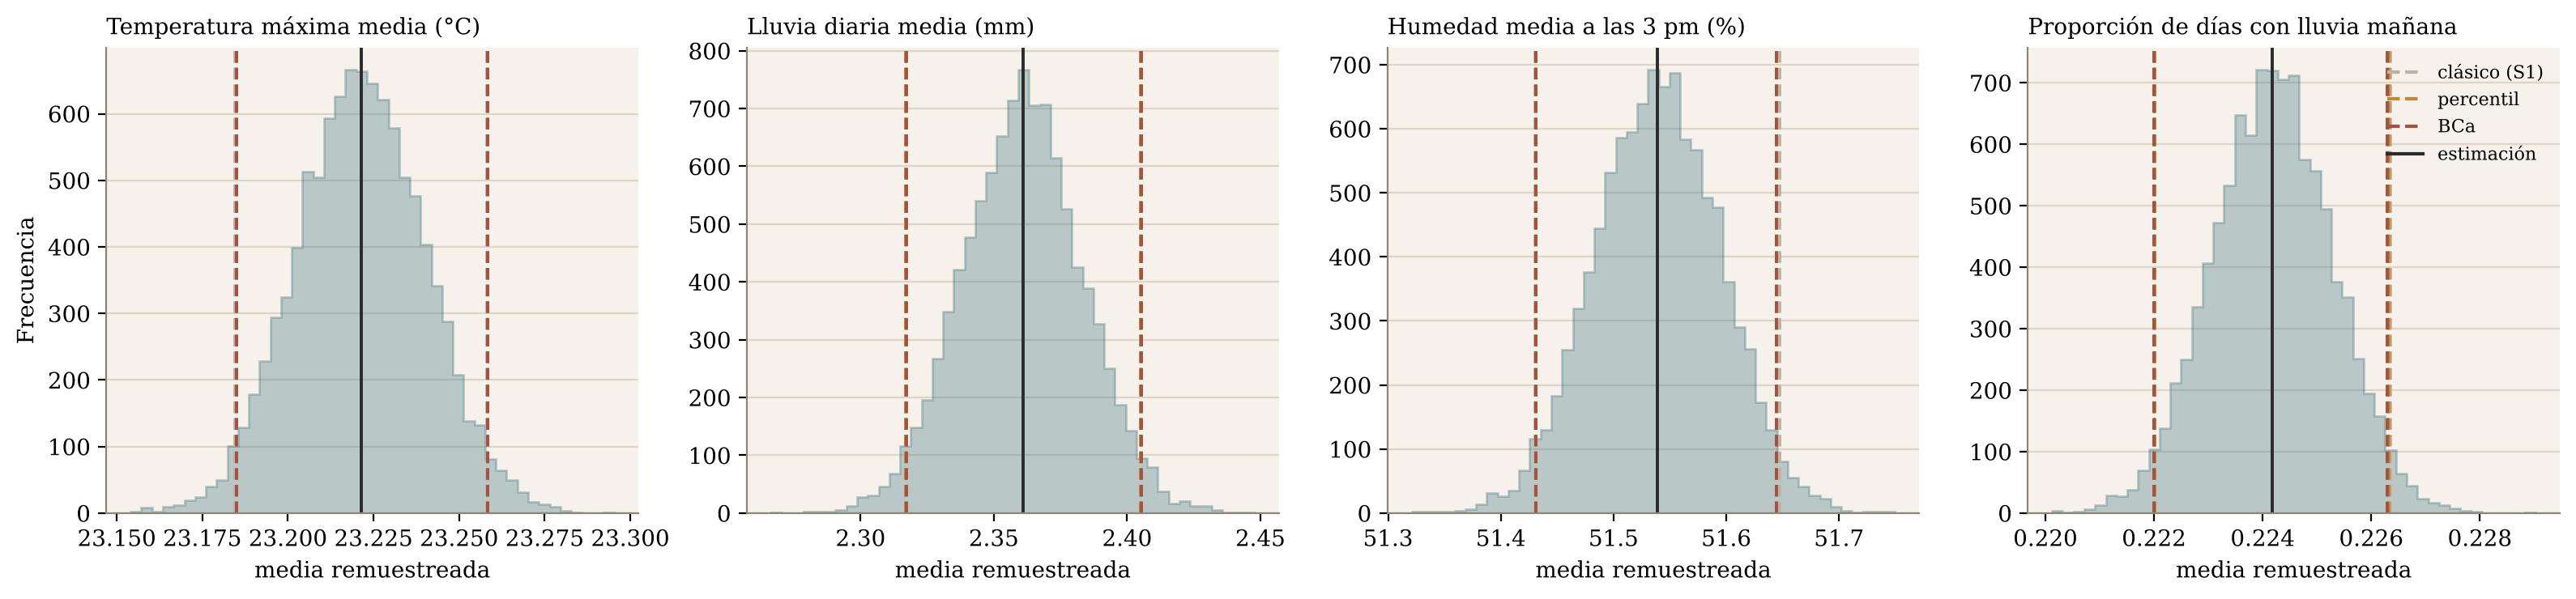
\includegraphics[width=\textwidth]{f2_fig_bootstrap.png}
\caption{Distribuciones bootstrap de los cuatro parámetros con los intervalos clásico, percentil y BCa (las líneas se superponen). La línea sólida es la estimación puntual.}
\end{figure}

En los cuatro parámetros los tres intervalos coinciden: $z_0$ está entre $-0{,}010$ y $0{,}002$ y $a$ es como máximo $0{,}004$. El caso con más corrección es la lluvia, la variable más asimétrica (mediana 0\,mm, máximo 371\,mm), pero su BCa se mueve menos de una milésima de mm. Esto pasa porque con más de 140.000 días la \textit{media muestral} sí es casi normal aunque la variable no lo sea (Teorema Central del Límite), como muestran los histogramas simétricos. Conclusión: los intervalos clásicos de la S1 son confiables. Eso no significa que la media de la lluvia sea un buen resumen de un día típico; lo revisamos en la Sección~\ref{sec:rob}.

\section{Validación de pruebas de hipótesis mediante permutación}
Validamos dos pruebas de la S1 con tests de permutación de 10.000 repeticiones (Good, 2005). Bajo $H_0$ da lo mismo qué días tienen la etiqueta ``llueve mañana'', así que mezclamos las etiquetas al azar, recalculamos el estadístico y contamos cuántas veces se iguala o supera el valor observado ($p = (k+1)/(B+1)$).

\begin{itemize}[leftmargin=1.2em,itemsep=0.2em]
\item \textbf{\textit{t} de Welch (humedad a las 3\,pm).} La humedad es 22,29 puntos más alta antes de un día con lluvia. Bajo $H_0$ la diferencia queda entre $-0{,}48$ y $0{,}48$ puntos (desv. est. 0,13).
\item \textbf{$\chi^2$ (nubosidad a las 3\,pm en tres tramos).} El estadístico observado es 10.812,6 ($n = 85.098$). Bajo $H_0$ nunca pasa de 18,0 (percentil 95 = 5,89).
\end{itemize}

\begin{figure}[H]
\centering
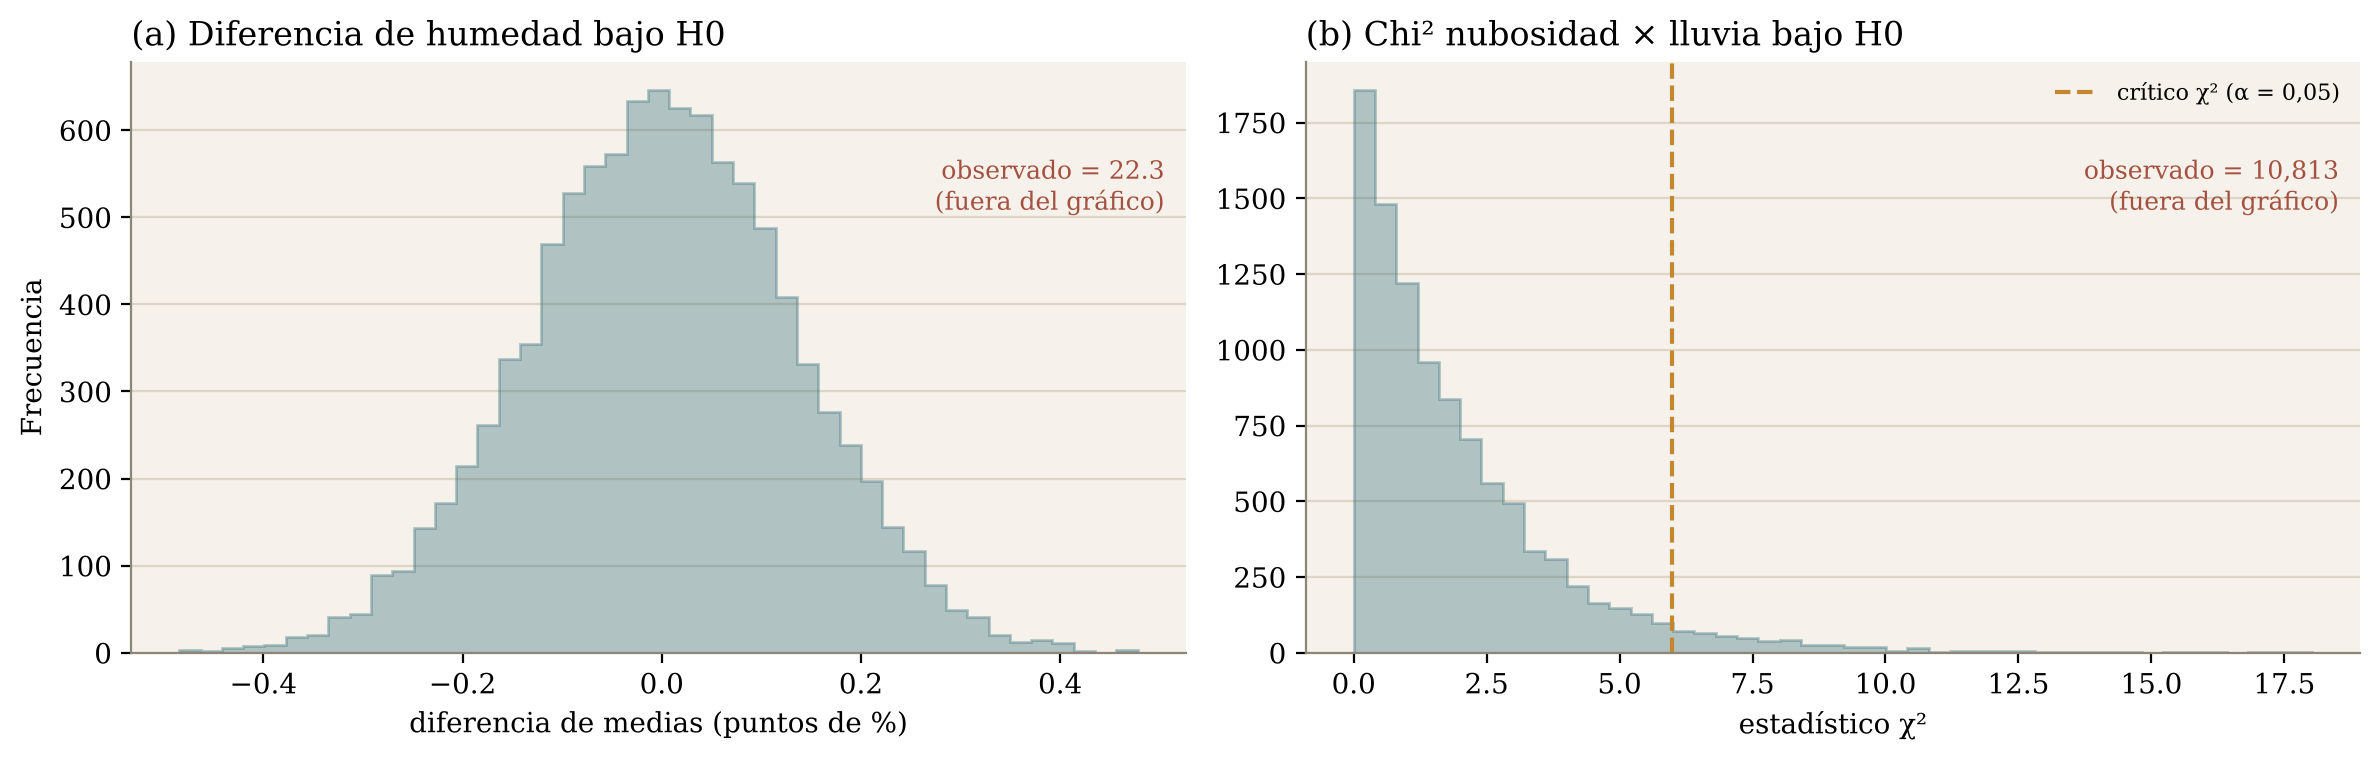
\includegraphics[width=0.92\textwidth]{f2_fig_permutacion.png}
\caption{Distribuciones bajo $H_0$ (10.000 permutaciones). En ambos casos el valor observado queda muy fuera del rango del azar.}
\end{figure}

Ninguna permutación alcanza el valor real, por lo que el valor $p$ de permutación es el mínimo posible con 10.000 repeticiones ($1/10.001 \approx 0{,}0001$), es decir, $p < 0{,}001$. Coincide con los resultados paramétricos de la S1 ($t = 182{,}6$; $\chi^2$ con 2 gl; ambos $p < 0{,}0001$). Los dos enfoques concuerdan y la permutación confirma que las conclusiones no dependían de la normalidad de la \textit{t} ni de la aproximación $\chi^2$.

\section{Evaluación de estabilidad de correlaciones}
Evaluamos cinco correlaciones de la S1 con intervalos bootstrap al 95\,\% (3.000 remuestras de filas). Incluimos a propósito una muy débil, para ver cómo se comporta. La correlación sol--nubosidad solo se calcula con las estaciones que miden ambas variables (64.892 días).

\begin{figure}[H]
\centering
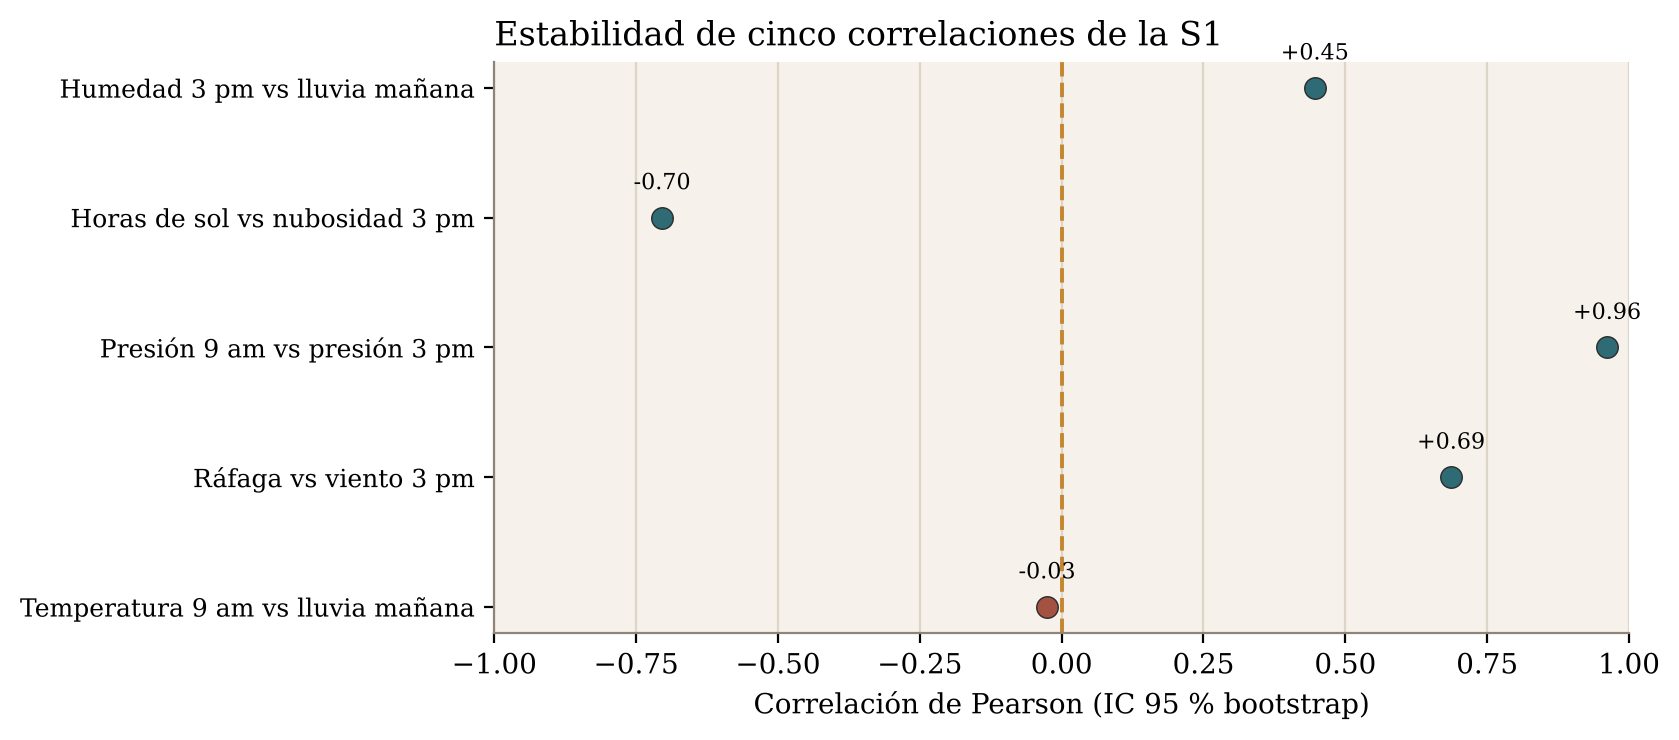
\includegraphics[width=0.78\textwidth]{f2_fig_correlaciones.png}
\caption{Intervalos bootstrap al 95\,\% de cinco correlaciones de la S1. Son tan estrechos que quedan tapados por el punto.}
\end{figure}

Las cinco son robustas: ningún intervalo cruza el cero y todos son muy estrechos. Humedad 3\,pm con lluvia mañana: $r = 0{,}446$ [0,442; 0,451]; sol con nubosidad: $-0{,}704$ [$-0{,}708$; $-0{,}701$]; presión 9\,am con 3\,pm: 0,961 [0,961; 0,962]; ráfaga con viento 3\,pm: 0,686 [0,683; 0,690]. La temperatura a las 9\,am con lluvia mañana ($r = -0{,}026$ [$-0{,}031$; $-0{,}021$]) también es estable, pero casi nula: con tantos datos hasta una relación sin importancia práctica tiene un intervalo que no toca el cero. La marcamos como \textit{robusta pero débil}.

\section{Simulación Monte Carlo basada en parámetros de S1}
\textbf{Pregunta de decisión:} al planificar un mes de trabajo al aire libre (una cosecha, una obra o un evento), ¿cuántos días de lluvia esperar y qué tan probable es una racha de varios días seguidos con lluvia? Usamos solo parámetros de la S1. La prueba \textit{z} mostró que la lluvia ``se arrastra'': si hoy llovió, mañana llueve con probabilidad $p_{11} = 0{,}464$; si no, con $p_{01} = 0{,}152$. Con esas dos probabilidades simulamos meses de 30 días, día a día, como una cadena de Markov (Robert \& Casella, 2004). Cada mes simulado es un dato sintético.

El modelo es coherente con los datos: la proporción de lluvia de largo plazo que implica, $\pi = p_{01}/(1-p_{11}+p_{01}) = 22{,}1\,\%$, es casi igual a la observada en la S1 (22,4\,\%). Simulamos 10.000 meses.

\begin{figure}[H]
\centering
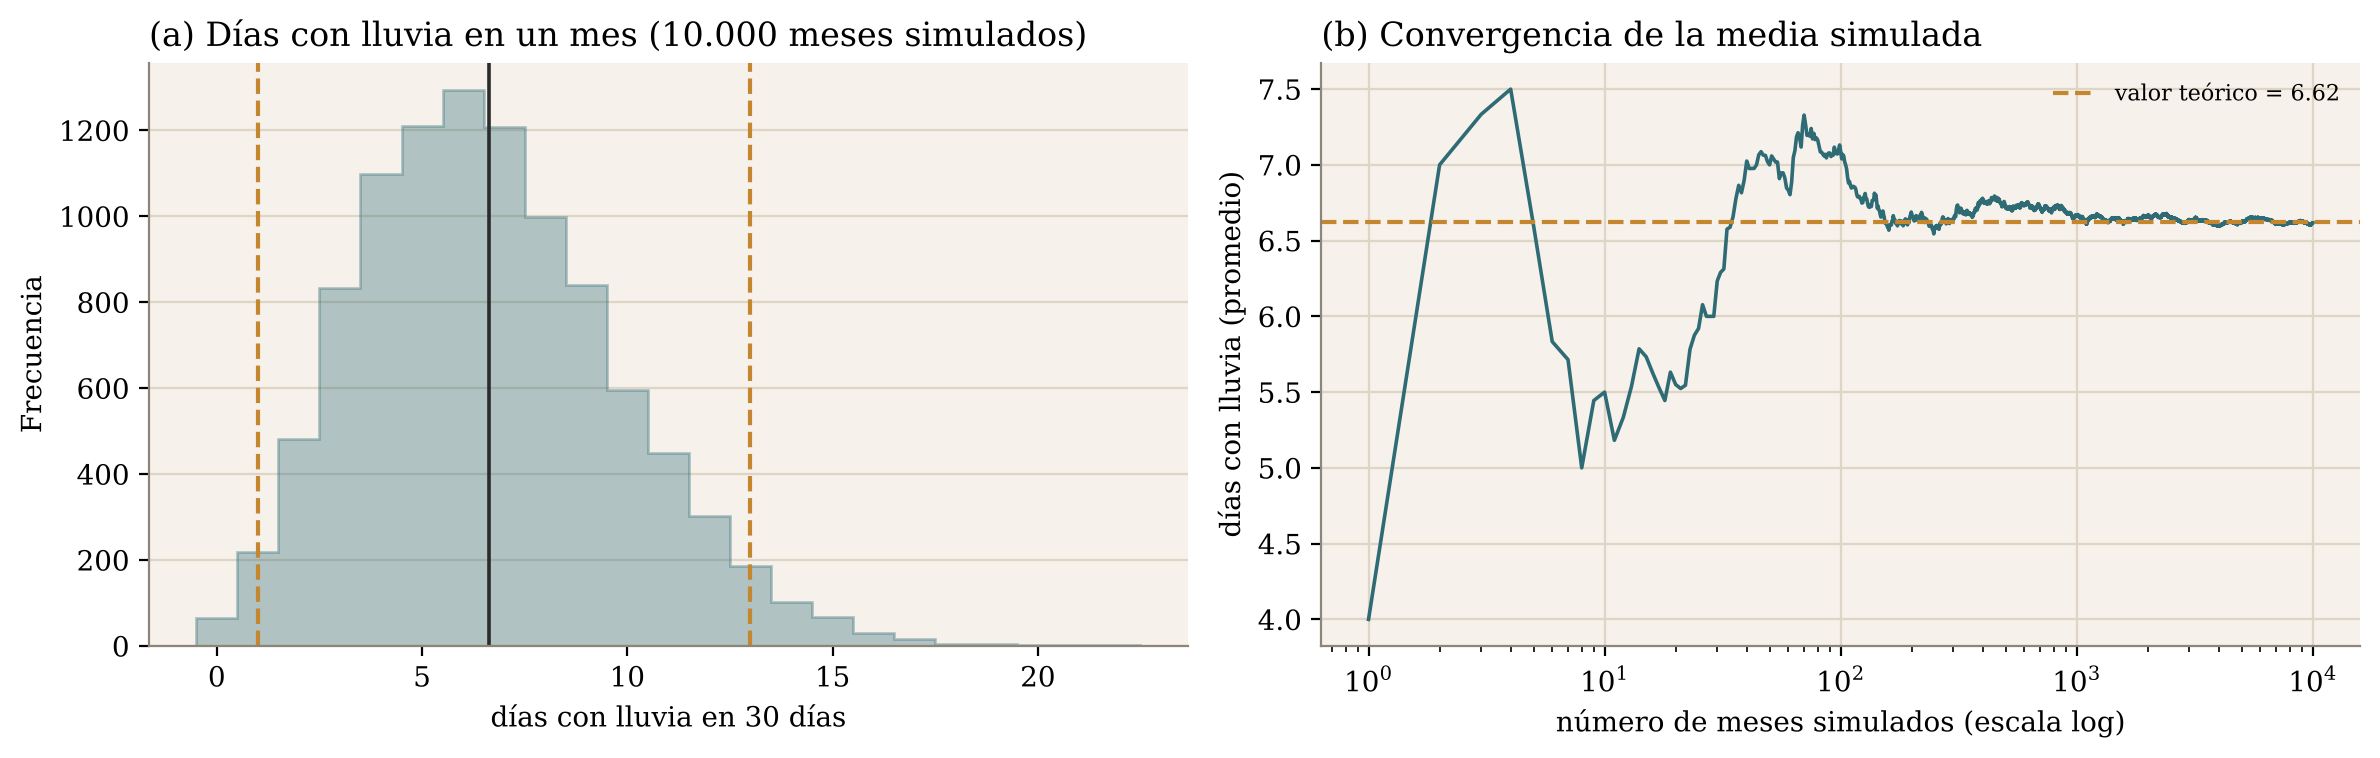
\includegraphics[width=0.92\textwidth]{f2_fig_montecarlo.png}
\caption{(a) Días con lluvia en 10.000 meses simulados, con el intervalo del 95\,\%. (b) Convergencia de la media simulada al valor teórico.}
\end{figure}

La media simulada es 6,62 días con lluvia por mes, igual al valor teórico ($30\pi$), y se estabiliza después de unos mil meses; con 10.000 el error estándar de Monte Carlo es de solo 0,03 días, así que las iteraciones son suficientes. El 95\,\% de los meses tiene entre 1 y 13 días con lluvia; hay un 17,6\,\% de probabilidad de 10 o más días, y un \textbf{55,7\,\%} de que haya al menos una racha de 3 o más días seguidos con lluvia. Un mes completo sin lluvia es muy raro (0,7\,\%).

\subsection{Escenarios: horizonte y supuesto de persistencia}
Repetimos la simulación para 7, 30 y 90 días y la comparamos con un modelo de días independientes (misma probabilidad media, sin persistencia).

\begin{table}[H]
\centering\small
\caption{Días con lluvia simulados (10.000 simulaciones por escenario).}
\begin{tabular}{@{}llrrcr@{}}
\toprule
Modelo & Días & Media & Desv. est. & IC 95\,\% & P(racha $\geq$ 3)\\
\midrule
Con persistencia (S1) & 7 & 1,55 & 1,44 & [0; 5] & 15,0\,\%\\
 & 30 & 6,62 & 3,11 & [1; 13] & 55,7\,\%\\
 & 90 & 19,92 & 5,41 & [10; 31] & 91,9\,\%\\
\midrule
Días independientes & 7 & 1,54 & 1,10 & [0; 4] & 3,9\,\%\\
 & 30 & 6,62 & 2,28 & [2; 11] & 21,2\,\%\\
 & 90 & 19,87 & 3,93 & [12; 28] & 53,6\,\%\\
\bottomrule
\end{tabular}
\end{table}

\begin{figure}[H]
\centering
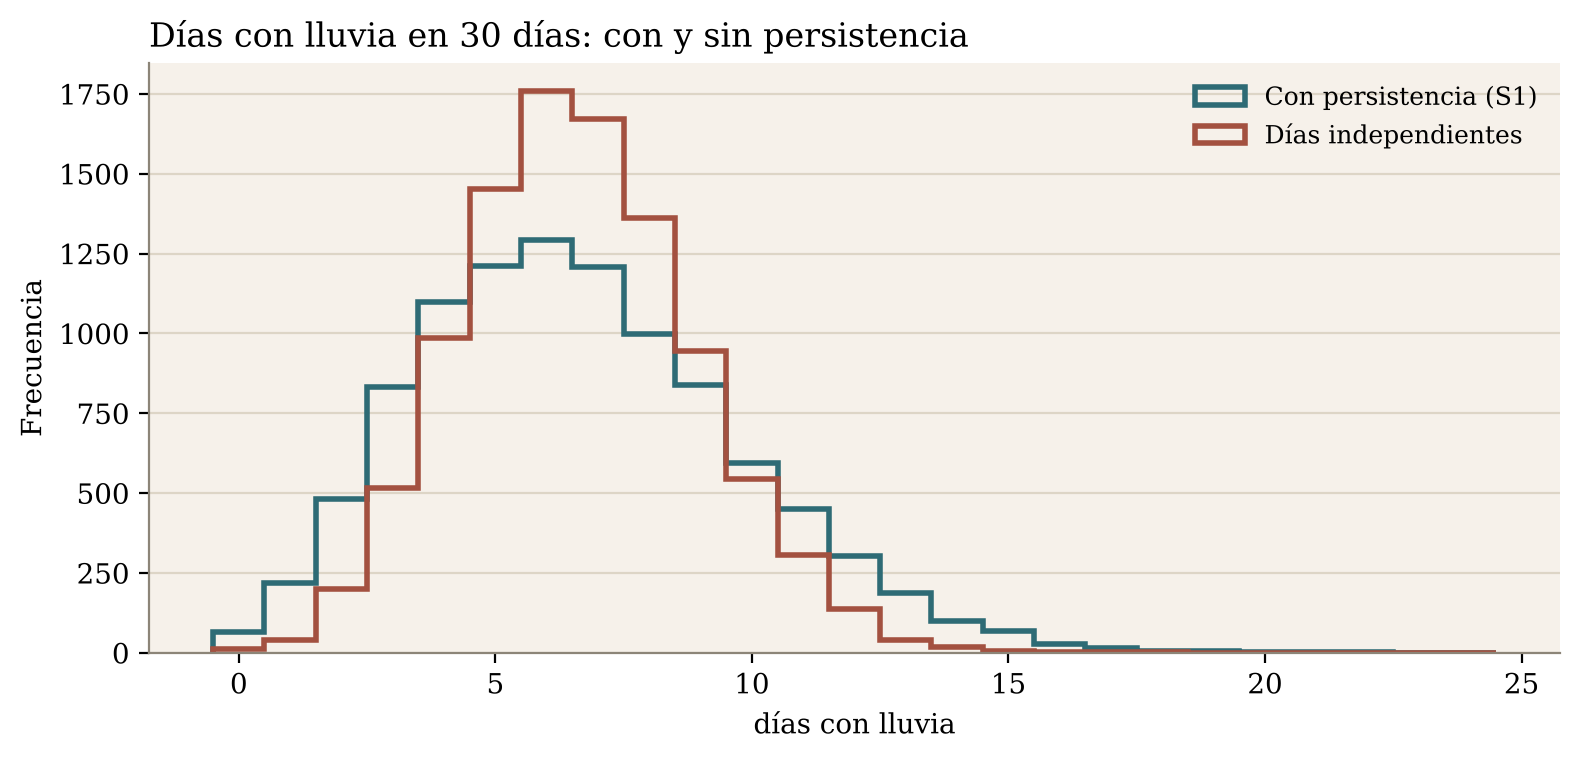
\includegraphics[width=0.66\textwidth]{f2_fig_escenarios.png}
\caption{Días con lluvia en 30 días con y sin persistencia: misma media, distinta dispersión.}
\end{figure}

La media es la misma en los dos modelos, pero el riesgo no: con persistencia los meses son más variables y la probabilidad de una racha de 3 o más días con lluvia sube de 21\,\% a 56\,\% (en 90 días, de 54\,\% a 92\,\%). Planificar suponiendo días independientes subestima el riesgo de varios días seguidos de lluvia, que es lo que más complica un trabajo al aire libre.

\section{Análisis de robustez}\label{sec:rob}
\textbf{Media de la lluvia y valores extremos.} La media (2,361\,mm) baja a 1,737\,mm al quitar solo el 1\,\% de días más lluviosos y a 0,975\,mm con la media recortada al 5\,\%; la mediana es 0\,mm. El error estándar jackknife (0,0225\,mm) es igual al clásico, así que el intervalo de la S1 es correcto, pero la media no representa un día típico: conviene usar la mediana o la proporción de días con lluvia. El día más influyente es el de 371\,mm.

\textbf{Supuesto de independencia.} En la S1 advertimos que los datos son días seguidos de las mismas 49 ciudades. Repetimos el bootstrap de la proporción de lluvia remuestreando ciudades completas: el intervalo pasa de [22,20\,\%; 22,63\,\%] a [20,55\,\%; 24,20\,\%], unas \textbf{8 veces más ancho}, porque la lluvia varía mucho entre ciudades (de 6,8\,\% en Woomera a 36,5\,\% en Portland). El 22,4\,\% es confiable como promedio, pero la incertidumbre real es mayor que la del intervalo clásico y no conviene aplicarlo a una ciudad en particular.

\textbf{Diferencia de humedad.} Con medianas da casi lo mismo que con medias (23,0 vs.\ 22,3 puntos) y es positiva en las 49 ciudades (de 6,6 a 33,3 puntos): no depende de unas pocas estaciones ni de valores extremos.

En síntesis, son confiables la diferencia de humedad, la asociación con la nubosidad (en las estaciones que la miden), las correlaciones y la persistencia de la lluvia. Requieren cautela la media de la lluvia y la precisión de la proporción global.

\section{Preparación para la Sumativa 3}
La Tabla~\ref{tab:val} resume qué resultados de la S1 quedaron validados (también en \path{data/processed/resultados_validados_f2.csv}).

\begin{table}[H]
\centering\small
\caption{Reporte de resultados validados.}
\label{tab:val}
\begin{tabular}{@{}>{\raggedright\arraybackslash}p{4.2cm}>{\raggedright\arraybackslash}p{6.3cm}>{\raggedright\arraybackslash}p{3.6cm}@{}}
\toprule
Resultado de S1 & Validación & Estado\\
\midrule
Temp. máxima y humedad medias & Clásico, percentil y BCa coinciden & Robusto\\
Lluvia diaria media & Intervalos coinciden; muy sensible a días extremos & Cautela: usar mediana\\
Proporción de lluvia mañana & IC por ciudad 8 veces más ancho; varía entre ciudades & Robusto como promedio\\
Welch humedad & Permutación $p<0{,}001$; se cumple en las 49 ciudades & Robusto\\
$\chi^2$ nubosidad & Permutación $p<0{,}001$; $\sim$40\,\% faltante no al azar & Robusto donde se mide\\
Correlaciones de la S1 & IC bootstrap estrechos, ninguno cruza 0 & Robustas (Temp.\ 9\,am débil)\\
Persistencia (46,4 vs.\ 15,2\,\%) & Monte Carlo reproduce la proporción observada & Robusto\\
\bottomrule
\end{tabular}
\end{table}

\textbf{Recomendaciones para la S3:} (1) usar como predictores las variables con relaciones robustas y fuertes: humedad a las 3\,pm, nubosidad, lluvia de hoy y presión; (2) no poner juntas variables casi repetidas (presión 9\,am y 3\,pm; ráfaga y viento 3\,pm; temperaturas máxima y de las 3\,pm); (3) describir la lluvia con la mediana o como variable binaria; (4) decidir cómo imputar \texttt{Sunshine} y \texttt{Cloud3pm}, muy útiles pero con 40--48\,\% de faltantes no al azar; (5) considerar la ciudad o zona y validar separando por ciudad o por tiempo, porque los días no son independientes; y (6) superar la línea base de 78\,\% de acierto de predecir siempre ``no llueve''.

\section*{Bibliografía}
\addcontentsline{toc}{section}{Bibliografía}
\small
\setlength{\parindent}{-1.2em}\setlength{\leftskip}{1.2em}
Efron, B. (1987). Better bootstrap confidence intervals. \textit{Journal of the American Statistical Association, 82}(397), 171--185. \url{https://doi.org/10.1080/01621459.1987.10478410}

Efron, B., \& Tibshirani, R. J. (1993). \textit{An introduction to the bootstrap}. Chapman \& Hall.

Good, P. I. (2005). \textit{Permutation, parametric, and bootstrap tests of hypotheses} (3.\textsuperscript{a} ed.). Springer.

Robert, C. P., \& Casella, G. (2004). \textit{Monte Carlo statistical methods} (2.\textsuperscript{a} ed.). Springer.

Virtanen, P., Gommers, R., Oliphant, T. E., Haberland, M., Reddy, T., Cournapeau, D., \ldots{} SciPy 1.0 Contributors. (2020). SciPy 1.0: Fundamental algorithms for scientific computing in Python. \textit{Nature Methods, 17}(3), 261--272. \url{https://doi.org/10.1038/s41592-019-0686-2}

Young, J. (2020). \textit{Rain in Australia} [Conjunto de datos]. Kaggle. \url{https://www.kaggle.com/datasets/jsphyg/weather-dataset-rattle-package}

\end{document}
